\documentclass[border=4pt]{standalone}
\usepackage{tikz}
\usepackage{xcolor}
\usepackage{pifont}
\usetikzlibrary{arrows.meta, positioning}
\begin{document}
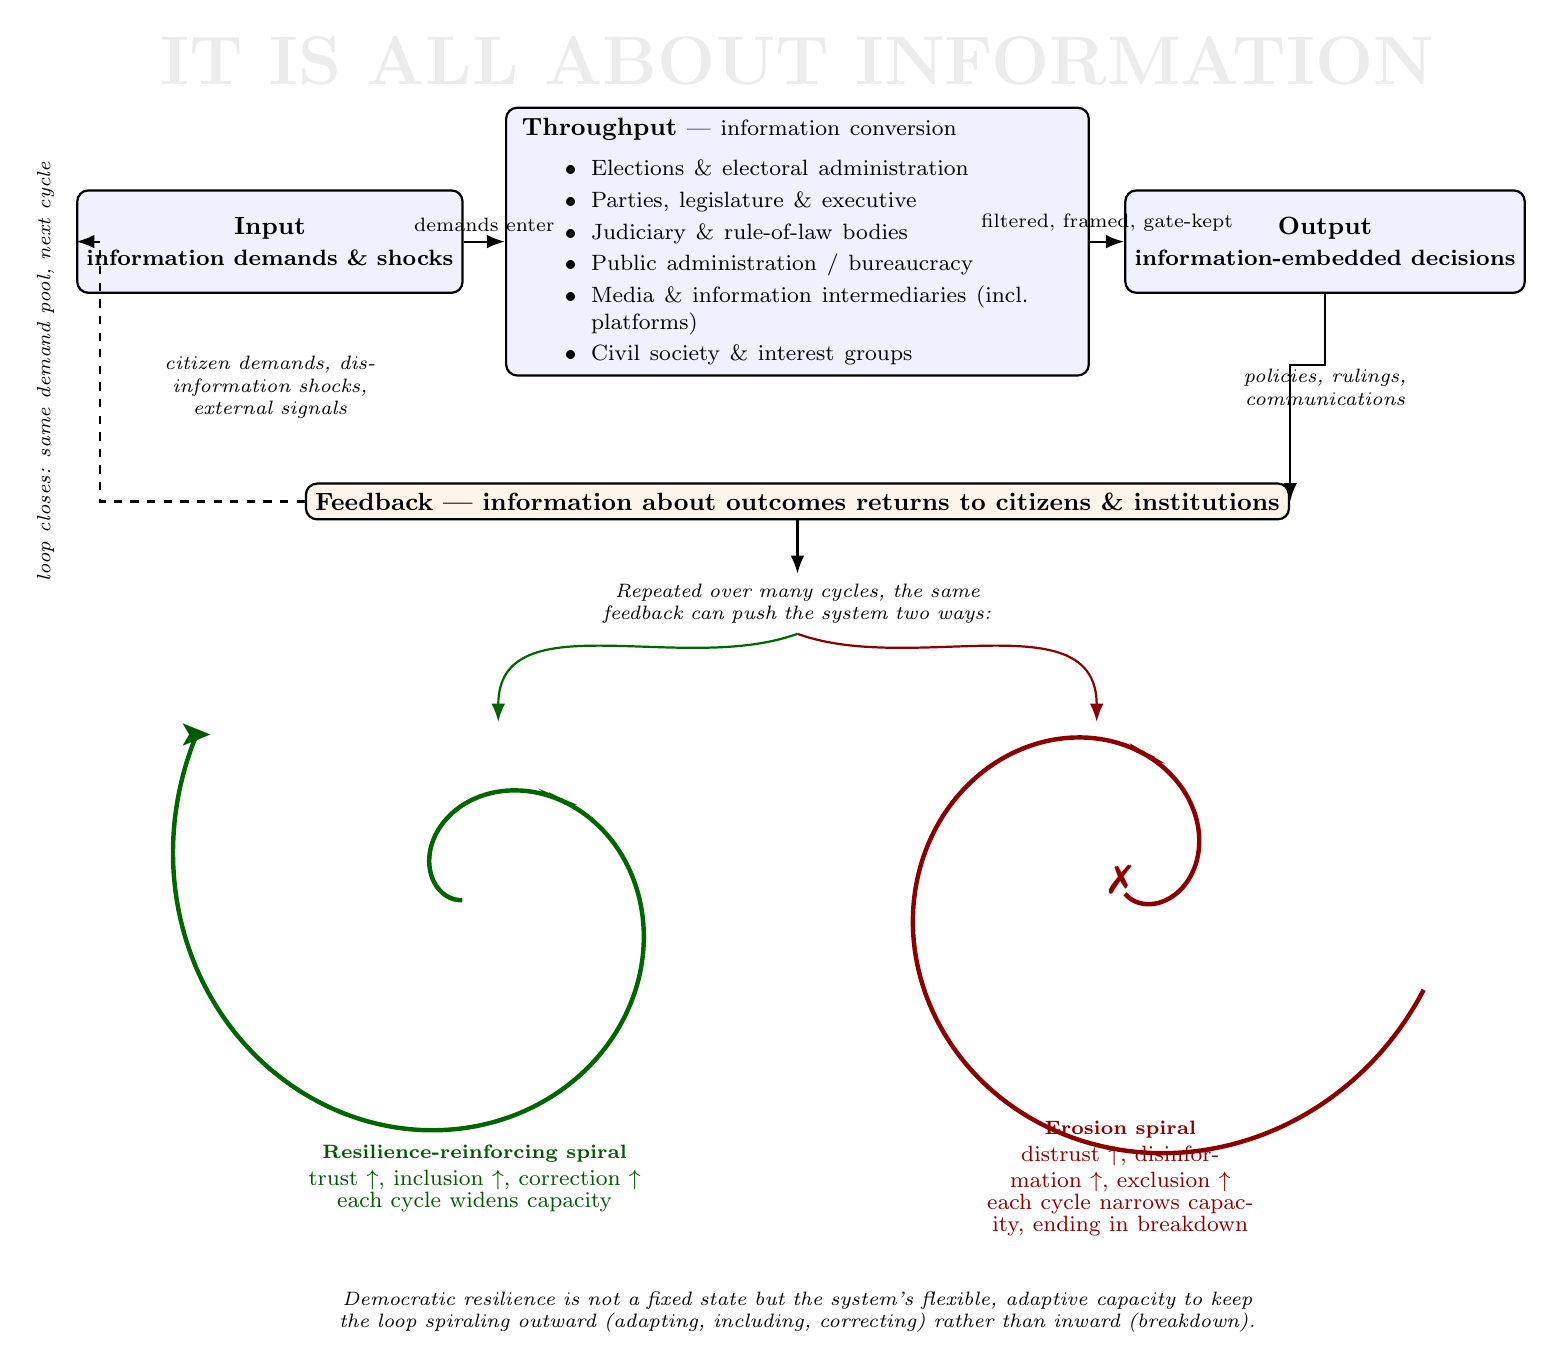
\begin{tikzpicture}[
  every node/.style = {font=\small},
  stage/.style   = {draw, rounded corners, align=center, fill=blue!6, minimum height=1.3cm, font=\bfseries\small},
  sub/.style     = {font=\scriptsize\itshape, text width=3.2cm, align=center},
  through/.style = {draw, rounded corners, align=left, fill=blue!6, minimum height=3.4cm, font=\bfseries\small},
  spiralcap/.style = {font=\bfseries\scriptsize, align=center},
  >=Latex, thick
]

% watermark
\node[font=\Huge\bfseries, text=gray!15] at (6.7,12.3) {IT IS ALL ABOUT INFORMATION};

% --- top row: Easton loop, information-relabelled ---
\node[stage, minimum width=3.2cm] (input) at (0,10) {Input\\\footnotesize information demands \& shocks};
\node[through, minimum width=7.4cm, text width=7cm] (through) at (6.7,10) {
  \bfseries\small Throughput \normalfont\footnotesize --- information conversion\\[2pt]
  \begin{itemize}\itemsep0pt\parsep0pt\topsep2pt\leftmargin=10pt
    \item Elections \& electoral administration
    \item Parties, legislature \& executive
    \item Judiciary \& rule-of-law bodies
    \item Public administration / bureaucracy
    \item Media \& information intermediaries (incl.\ platforms)
    \item Civil society \& interest groups
  \end{itemize}
};
\node[stage, minimum width=3.2cm] (output) at (13.4,10) {Output\\\footnotesize information-embedded decisions};

\draw[->] (input) -- node[above,font=\scriptsize]{demands enter} (through);
\draw[->] (through) -- node[above,font=\scriptsize]{filtered, framed, gate-kept} (output);

\node[sub] at (0,8.15) {citizen demands, disinformation shocks, external signals};
\node[sub] at (13.4,8.15) {policies, rulings, communications};

% --- feedback node ---
\node[draw, rounded corners, fill=orange!8, font=\bfseries\small, align=center, minimum width=6.5cm] (fb) at (6.7,6.7) {Feedback --- information about outcomes returns to citizens \& institutions};
\draw[->] (output.south) -- ++(0,-0.9) -| (fb.east);
\draw[->, dashed] (fb.west) -- ++(-2.6,0) |- (input.west);
\node[font=\scriptsize\itshape, rotate=90] at (-2.85,8.35) {loop closes: same demand pool, next cycle};

\node[font=\scriptsize, align=center, text width=8cm] (hub) at (6.7,5.4) {\textit{Repeated over many cycles, the same feedback can push the system two ways:}};
\draw[->, thick] (fb.south) -- (hub.north);

% --- two spirals ---
\draw[->, green!40!black, thick] (hub.south) to[out=200,in=90] (2.9,3.9);
\draw[->, red!55!black, thick] (hub.south) to[out=-20,in=90] (10.5,3.9);

\coordinate (gc) at (2.6,1.7);
\coordinate (rc) at (10.8,1.9);

% green: resilience-reinforcing, expands outward over cycles
\draw[green!40!black, ultra thick, rounded corners=1pt]
  plot[domain=0:410, samples=180, smooth, variable=\t]
  ({2.6 + (0.18+0.0095*\t)*cos(200-\t)}, {1.7 + (0.18+0.0095*\t)*sin(200-\t)});
\node[green!35!black, font=\bfseries\large] at ({2.6 + (0.18+0.0095*410)*cos(200-410)}, {1.7 + (0.18+0.0095*410)*sin(200-410)}) {\ding{228}};

% red: erosion, collapses inward over cycles
\draw[red!55!black, ultra thick, rounded corners=1pt]
  plot[domain=0:410, samples=180, smooth, variable=\t]
  ({10.8 + (4.1-0.0095*\t)*cos(-20-\t)}, {1.9 + (4.1-0.0095*\t)*sin(-20-\t)});
\node[red!55!black, font=\bfseries\Large] at (rc) {\ding{55}};

\node[spiralcap, green!35!black, text width=4.8cm] at (2.6,-1.9) {Resilience-reinforcing spiral\\\footnotesize\normalfont trust $\uparrow$, inclusion $\uparrow$, correction $\uparrow$\\ each cycle widens capacity};
\node[spiralcap, red!55!black, text width=4.8cm] at (10.8,-1.9) {Erosion spiral\\\footnotesize\normalfont distrust $\uparrow$, disinformation $\uparrow$, exclusion $\uparrow$\\ each cycle narrows capacity, ending in breakdown};

\node[font=\scriptsize\itshape, align=center, text width=13.5cm] at (6.7,-3.6) {Democratic resilience is not a fixed state but the system's flexible, adaptive capacity to keep the loop spiraling outward (adapting, including, correcting) rather than inward (breakdown).};

\end{tikzpicture}
\end{document}
